\newpage
\section*{Esempi}
\textbf{Qui trovi alcune prove ed esempi di come mettere le immagini.}

\begin{figure}[h]
    \centering
    \begin{subfigure}[]{0.5\linewidth}
    \centering
    
\includegraphics[scale=0.2]{img/pittogrammi/Acute toxicity.png}
    \caption{Acute toxicity}
    \end{subfigure}
    \begin{subfigure}[]{0.5\linewidth}
    \centering
    
\includegraphics[scale=0.2]{img/pittogrammi/Explosive.png}
    \caption{Explosive}
    \end{subfigure}
    \caption{Due immagini incolonnate al centro della pagina con posizione h definita da te.}
    \label{fig:1}
\end{figure}

\textit{Lorem ipsum dolor sit amet, consectetur adipiscing elit. Maecenas eget nisl elementum, pretium libero suscipit, interdum tellus. Praesent luctus commodo massa, vel molestie augue laoreet ac. Phasellus sodales auctor erat eu porta. Donec at volutpat nunc. Phasellus pretium, eros vitae cursus ornare, turpis massa egestas sem, ut varius ipsum metus nec mi. Integer ut odio erat. Interdum et malesuada fames ac ante ipsum primis in faucibus. Sed finibus, tortor in tristique iaculis, odio tortor finibus nisi, nec varius felis justo eu tortor. Interdum et malesuada fames ac ante ipsum primis in faucibus. Donec ultrices in ante vel imperdiet. Ut porttitor consectetur sodales. Vestibulum ante ipsum primis in faucibus orci luctus et ultrices posuere cubilia curae; Nullam non neque quis tortor convallis pulvinar id vel libero.}

\begin{figure}[!h]
\floatbox[{\capbeside\thisfloatsetup{capbesideposition={right,top},capbesidewidth=0.45\textwidth}}]{figure}[\FBwidth]
{\caption{didascalia dell'immagine centrale con didascalia a fianco.}}
{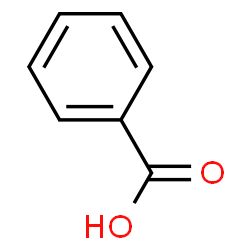
\includegraphics[width=0.1\textwidth]{img/acbenz.png}}
{\label{fig:2}}
\end{figure}

\textit{Aliquam erat nulla, suscipit id dignissim molestie, eleifend quis tortor. Pellentesque tempus egestas orci, sit amet eleifend elit condimentum id. Etiam id nisi velit. Etiam mauris nisl, facilisis sed egestas nec, tempor a est. In eget lacus vitae velit volutpat maximus. Vestibulum maximus arcu sit amet lacus maximus consequat. Duis sodales libero non metus finibus, eget ornare sem consequat.}

\begin{wrapfigure}{r}{0.3\textwidth} %this figure will be at the right
    \centering
    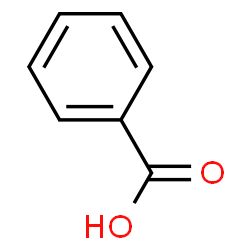
\includegraphics[scale=0.5]{img/acbenz.png}
    \caption{Didascalia dell'immagine sulla destra circondata da testo.} 
    \label{fig:3}
\end{wrapfigure}

\textit{Nullam vel lorem porttitor, convallis ex eget, condimentum velit. Integer sed sem aliquet, elementum ipsum in, rutrum elit. Vestibulum in arcu eget odio egestas varius. Vivamus lacus augue, dignissim at arcu a, consequat iaculis leo. Nam sit amet varius tellus. Nulla tempor velit nibh, et tincidunt diam porta vel. Mauris sit amet erat ut neque vehicula ultrices et eu sem. Phasellus pellentesque ultricies sapien. Curabitur at sodales mauris, maximus auctor mi. Vestibulum semper mauris in euismod rutrum. Fusce pellentesque in mi ac euismod.}

\textit{Nam gravida magna ut volutpat placerat. Pellentesque habitant morbi tristique senectus et netus et malesuada fames ac turpis egestas. Sed consequat justo condimentum metus bibendum mattis. Etiam id euismod ante. Nam sit amet ex libero. Proin id mauris at neque pellentesque accumsan eu ut ligula. Vivamus sodales magna sed risus faucibus tincidunt in eu felis.}

\begin{figure}
    \centering
    
\includegraphics[scale=0.2]{img/pittogrammi/Acute toxicity.png}
    
\includegraphics[scale=0.2]{img/pittogrammi/Explosive.png}
    \caption{Figure affiancate al centro della pagina nella posizione decisa da LaTex}
    \label{fig:4}
\end{figure}

\textit{Vivamus sit amet suscipit turpis, at eleifend risus. Vestibulum ante ipsum primis in faucibus orci luctus et ultrices posuere cubilia curae; Curabitur eget pharetra est, in mattis erat. Aenean pharetra finibus posuere. Nullam ipsum lacus, molestie nec eros eu, lacinia facilisis augue. Aenean dapibus rhoncus mi ut vulputate. Mauris commodo ultricies nulla egestas porttitor.}

\begin{figure}[h]
    \centering
    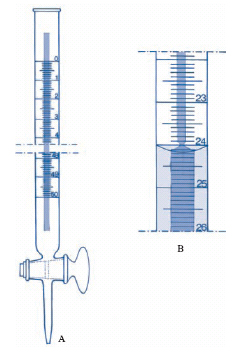
\includegraphics{img/buretta.jpg}
    \caption{Buretta}
    \label{fig:5}
\end{figure}



Adesso provo a fare un commit su Git.
